ROS (Robotic Operating System) is an open source framework made toward robotic application.
The goal of ROS is to propose means to facilitate communication between processes,managing possibilities and make available working algorithms for everyone~\cite{quigley2009ros}.

This framework will be use in this project for communication and visualisation.

\subsection{How it works}

ROS is functioning with nodes, a master and slaves,the master is a ROS process and nodes can be programmed by anyone:

\begin{itemize}[label=$-$,itemsep=0cm,topsep=0cm]
\item The framework is available on many OS (operating system)such as Linux (CPU architecture: ARM x86 x64), Android , Windows, OSX;
\item The programming of the nodes can be done in multiple language : C++, Python, Java, Lua, Lisp, C\#, Go, R, Ruby (from the most supported to the least)
\item Nodes written in different languages can function together.
\end{itemize}

The communication with ROS works with topics,subscriber, and publisher, a publishing node will announce to the master that it is publishing over a topic and the subscribing node will say to the master that it want to listen to a topic. Then if the publisher and the subscriber are on the same topic, the master will transfer data in order for the two other node to communicate directly via TCP/IP or UDP (see figure~\ref{fig:rosTopic}).

\begin{figure}[H]
\centering
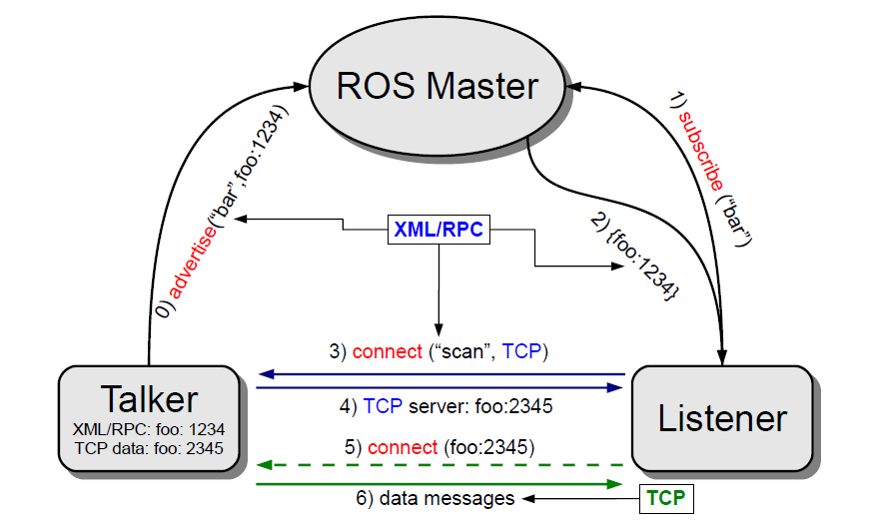
\includegraphics[scale=0.75]{ros_func.png}
\caption{Connection of nodes and topics \cite{rusu13ros}.}
\label{fig:rosTopic}
\end{figure}

ROS also facilitate the serialization of messages (conversion of the message into bytes):\\

\begin{minipage}[b]{0.8\textwidth}
\begin{itemize}[label={},itemsep=0cm,topsep=0cm]
\item std\_msgs/Header header
  \begin{itemize}[label={},itemsep=0cm,topsep=0cm]
  \item uint32 seq
  \item time stamp
  \item string frame\_id
   \end{itemize}
\item geometry\_msgs/Quaternion orientation
  \begin{itemize}[label={},itemsep=0cm,topsep=0cm]
  \item float64 x
  \item float64 y
  \item float64 z
  \item float64 w
  \end{itemize}
\end{itemize}
\end{minipage}


As it can be seen in the message example, a message can reference another message, in order to create message capable of transmitting complex data (an image with all its meta data).
This functionality of ROS permits a big modularity for the programmer, an easy passage from simulation to real via only changing topic names.

\subsection{ROS in the project}

For the simulation of the swarm slam project multiple nodes have been
created in order to represent accurate communication and sensing.

\subsubsection*{IA\_MSGS}

ia\_msgs is a utility package to regroup created message to help to the communication of interval vector (in 2 and 3 dimension):\\

ia\_msgs/StampedInterval
\begin{itemize}[label={},itemsep=0cm,topsep=0cm]
\item std\_msgs/Header header
  \begin{itemize}[label={},itemsep=0cm,topsep=0cm]
  \item uint32 seq
  \item time stamp
  \item string frame\_id
  \end{itemize}
\item ia\_msgs/IdInterval[] data
  \begin{itemize}[label={},itemsep=0cm,topsep=0cm]
  \item uint8 id
  \item ia\_msgs/Interv[] data
    \begin{itemize}[label={},itemsep=0cm,topsep=0cm]
    \item geometry\_msgs/Point position
      \begin{itemize}[label={},itemsep=0cm,topsep=0cm]
      \item float64 x
      \item float64 y
      \item float64 z
      \end{itemize}
    \item float64 width
    \item float64 height
    \end{itemize}
  \end{itemize}
\end{itemize}

The above message allows to send with a time stamp and a reference frame a list of an identified list of two-dimensional boxes,it is used to send the estimates of the beacons.

\subsubsection*{RVIZ\_IA\_PLUGIN}

The rviz plug-in has been done to ease the visualization of the interval, rviz is on openGL based graphic visualizer incorporated in ROS. rviz can receive message and interpret them.

\begin{figure}[H]
\centering
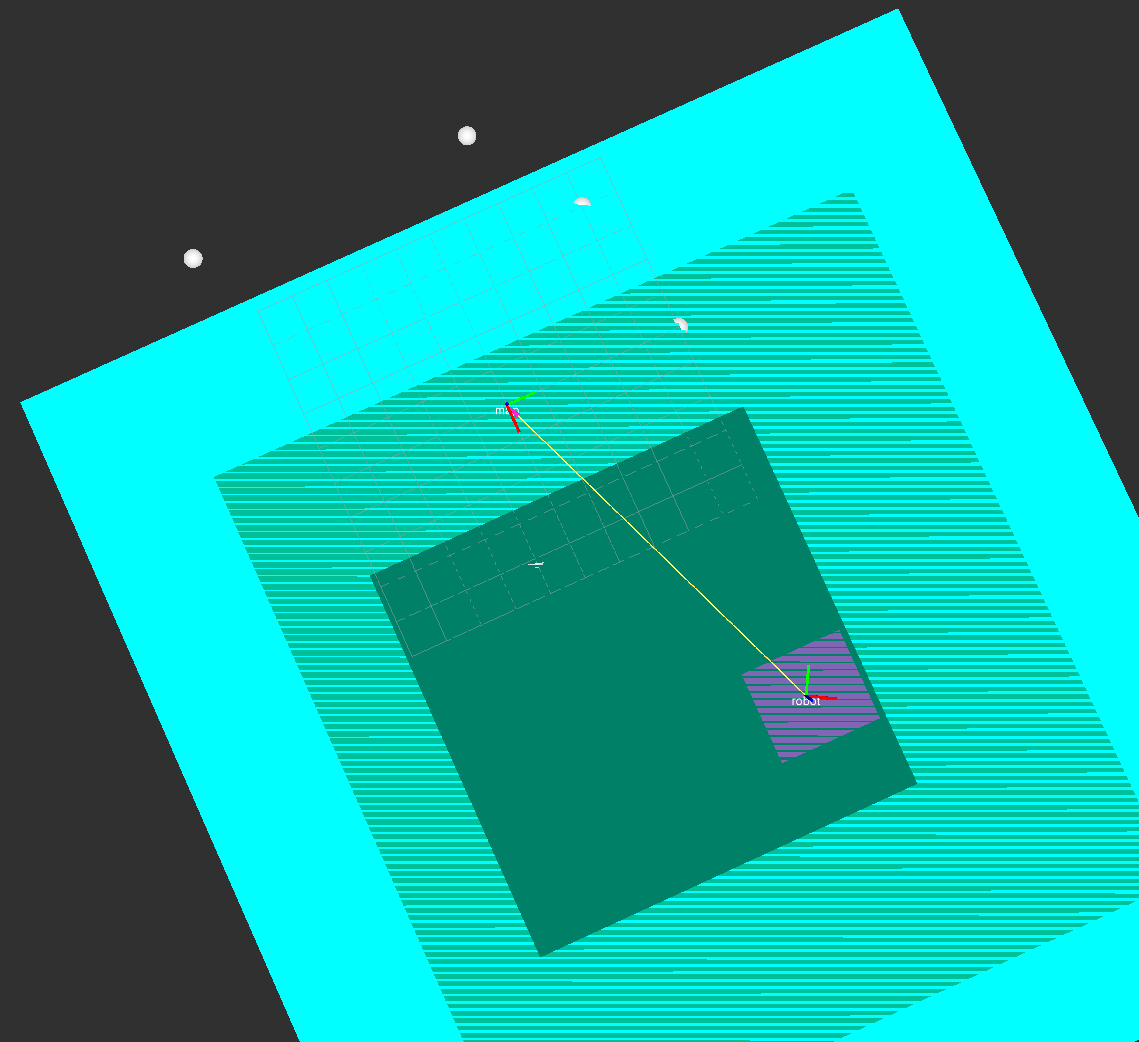
\includegraphics[scale=0.13,angle=0]{picture_no_sivia.png}
\caption{Example of rviz utilisation.}
\label{fig:rvizEx}
\end{figure}

In figure~\ref{fig:rvizEx} rviz interpret the StampedInterval message (the blue rectangle), two frame, the real pose of the robot and the map frame seen as an ensemble of blue, green and red arrow, the point cloud of beacons printed as spheres and the Interval message for the pose estimate of the robot.
What has been done is the interpretation of the interval related messages.

\subsubsection*{IA\_SLAM}

It is the core of the project this node receive the sensor data (distance from the beacons), the information from other robots and the proprioceptive data such as the heading,speed motors order, then it estimate the position of the robot and the beacons by using the algorithm from the section~\ref{sec:slamtheory}.It has been implemented in C++ as it create an heavy load on the CPU.

The arithmetic of intervals is done with the help of the IBEX library a C++ library towards intervals applications~\cite{ibex}
\subsubsection*{ROBOT\_SIMU}

This node simulates the robot by using the state equation (a car model for the project) its send the pose information to the beacon\_simu node and the proprioceptive information to the ia\_slam node.This node and all the other simulation nodes have been implemented in Python for easier manipulation.

\subsubsection*{BEACON\_SIMU}

This node simulates the sensor of the beacons,it knows the real pose of the beacons and the pose of the robot and considering the distance from the beacons it send or not the information every second (ia\_slam received a beacon data every tenth of a second).

\subsubsection*{TALK\_SIMU}

This node works on the same principle as the beacon\_simu node but for the discussion between robots, if the robots are close enough data is transferred with a limitation in time,a transfer can only happened three seconds after another to model the bandwidth limitation with underwater modem, the time was chosen arbitrarily but can be quickly changed.

\subsubsection*{IA\_CONTROLLER}

This node is receiving the position of the robot and the other robots, in order to compute the motors orders to follow the path and avoid obstacles. The orders are then sent to the robot\_simu node.

\begin{figure}[H]
\centering
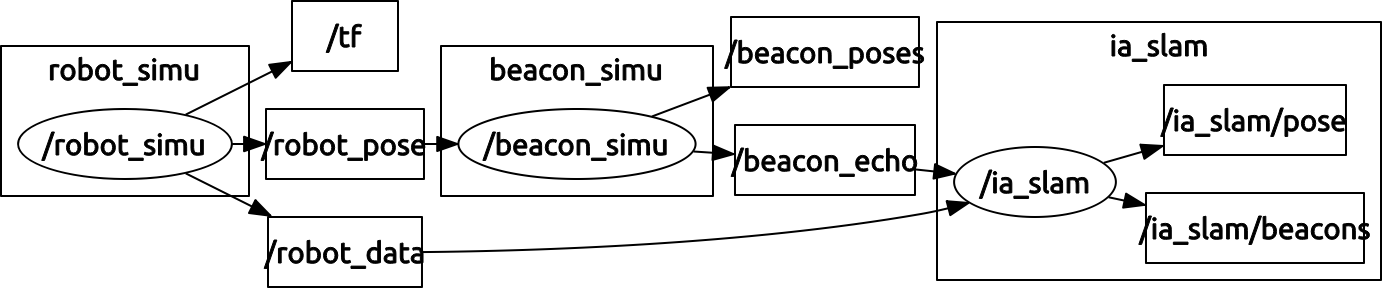
\includegraphics[scale=0.3,angle=0]{simple_slam_ros.png}
\caption{Relation between nodes with one robot and no controller node.}
\label{fig:oneRobGraph}
\end{figure}

In figure~\ref{fig:oneRobGraph} is represented the relation between nodes with only one robots with the help of rqt\_graph, a ROS program. A  similar graph can be found in the appendix (figure~\ref{fig:completeNode}).